% !TeX program = pdflatex
% Compilar desde la raíz: latexmk -cd -pdf informe/Ficha_Proyecto_ES_EN.tex
\documentclass[10pt,a4paper]{article}
\usepackage[margin=16mm,top=19mm,bottom=17mm,headheight=24pt]{geometry}
\usepackage{iftex}
\ifPDFTeX
  \usepackage[T1]{fontenc}
  \usepackage[utf8]{inputenc}
  \usepackage{lmodern}
  \renewcommand{\familydefault}{\sfdefault}
\else
  \usepackage{fontspec}
  \IfFontExistsTF{DejaVu Sans}{\setmainfont{DejaVu Sans}\setsansfont{DejaVu Sans}}{\setmainfont{Latin Modern Sans}\setsansfont{Latin Modern Sans}}
\fi
\usepackage[spanish,es-tabla]{babel}
\usepackage{graphicx,xcolor,tikz,tabularx,array,booktabs,enumitem,tcolorbox,fancyhdr,hyperref,xurl,microtype,multicol,etoolbox}
\graphicspath{{informe/}{./}}
\usetikzlibrary{arrows.meta,positioning,shapes.geometric,calc,babel}
\definecolor{navy}{HTML}{091B36}\definecolor{blue}{HTML}{0965EB}\definecolor{cyan}{HTML}{00A9E8}\definecolor{muted}{HTML}{536782}\definecolor{light}{HTML}{F1F6FD}\definecolor{line}{HTML}{DBE5F2}\definecolor{white}{HTML}{FFFFFF}\definecolor{ink}{HTML}{1D2C46}
\hypersetup{colorlinks=true,urlcolor=blue,linkcolor=blue,pdftitle={ASTROVITAL | Ficha del Proyecto},pdfauthor={ASTROVITAL}}
\setlength{\parindent}{0pt}\setlength{\parskip}{5.2pt}\linespread{1.04}
\setlist[itemize]{leftmargin=5mm,itemsep=2.1pt,topsep=3pt,parsep=0pt}
\pagestyle{fancy}\fancyhf{}\renewcommand{\headrulewidth}{0pt}
\fancyhead[L]{
\includegraphics[width=27mm]{astrovital_logo_claro.png}}\fancyhead[R]{\footnotesize\bfseries\color{muted}FICHA TÉCNICA · ASTROVITAL}
\fancyfoot[L]{\color{muted}\scriptsize ASTROVITAL \quad | \quad MONITOREO DE SALUD ESPACIAL}
\fancyfoot[R]{\color{blue}\bfseries\small\thepage}
\newcommand{\heading}[2]{\par\vspace{8pt}{\large\bfseries\color{navy}#1}\hfill{\footnotesize\bfseries\color{blue}#2}\par\vspace{-1pt}{\color{blue}\rule{\linewidth}{1pt}}\vspace{3pt}}
\newcommand{\tinyhead}[1]{{\footnotesize\bfseries\color{blue}\MakeUppercase{#1}}}
\newtcolorbox{infobox}[1][]{colback=light,colframe=line,boxrule=.5pt,arc=1.5mm,left=9pt,right=9pt,top=8pt,bottom=8pt,#1}
\newtcolorbox{navybox}[1][]{colback=navy,colframe=navy,boxrule=0pt,arc=1.8mm,left=12pt,right=12pt,top=10pt,bottom=10pt,#1}
\newcommand{\linktxt}[2]{\href{#2}{\textcolor{blue}{\bfseries #1}}}
\newcommand{\field}[2]{{\tinyhead{#1}}\par{\bfseries\color{navy}#2}}
\begin{document}
\thispagestyle{empty}
% Fotografía de portada suministrada por el equipo.
\AddToHookNext{shipout/background}{%
\begin{tikzpicture}[remember picture,overlay]
\begin{scope}
\clip (current page.north west) rectangle ([yshift=-157mm]current page.north east);
\node[anchor=north,inner sep=0pt] at (current page.north)
{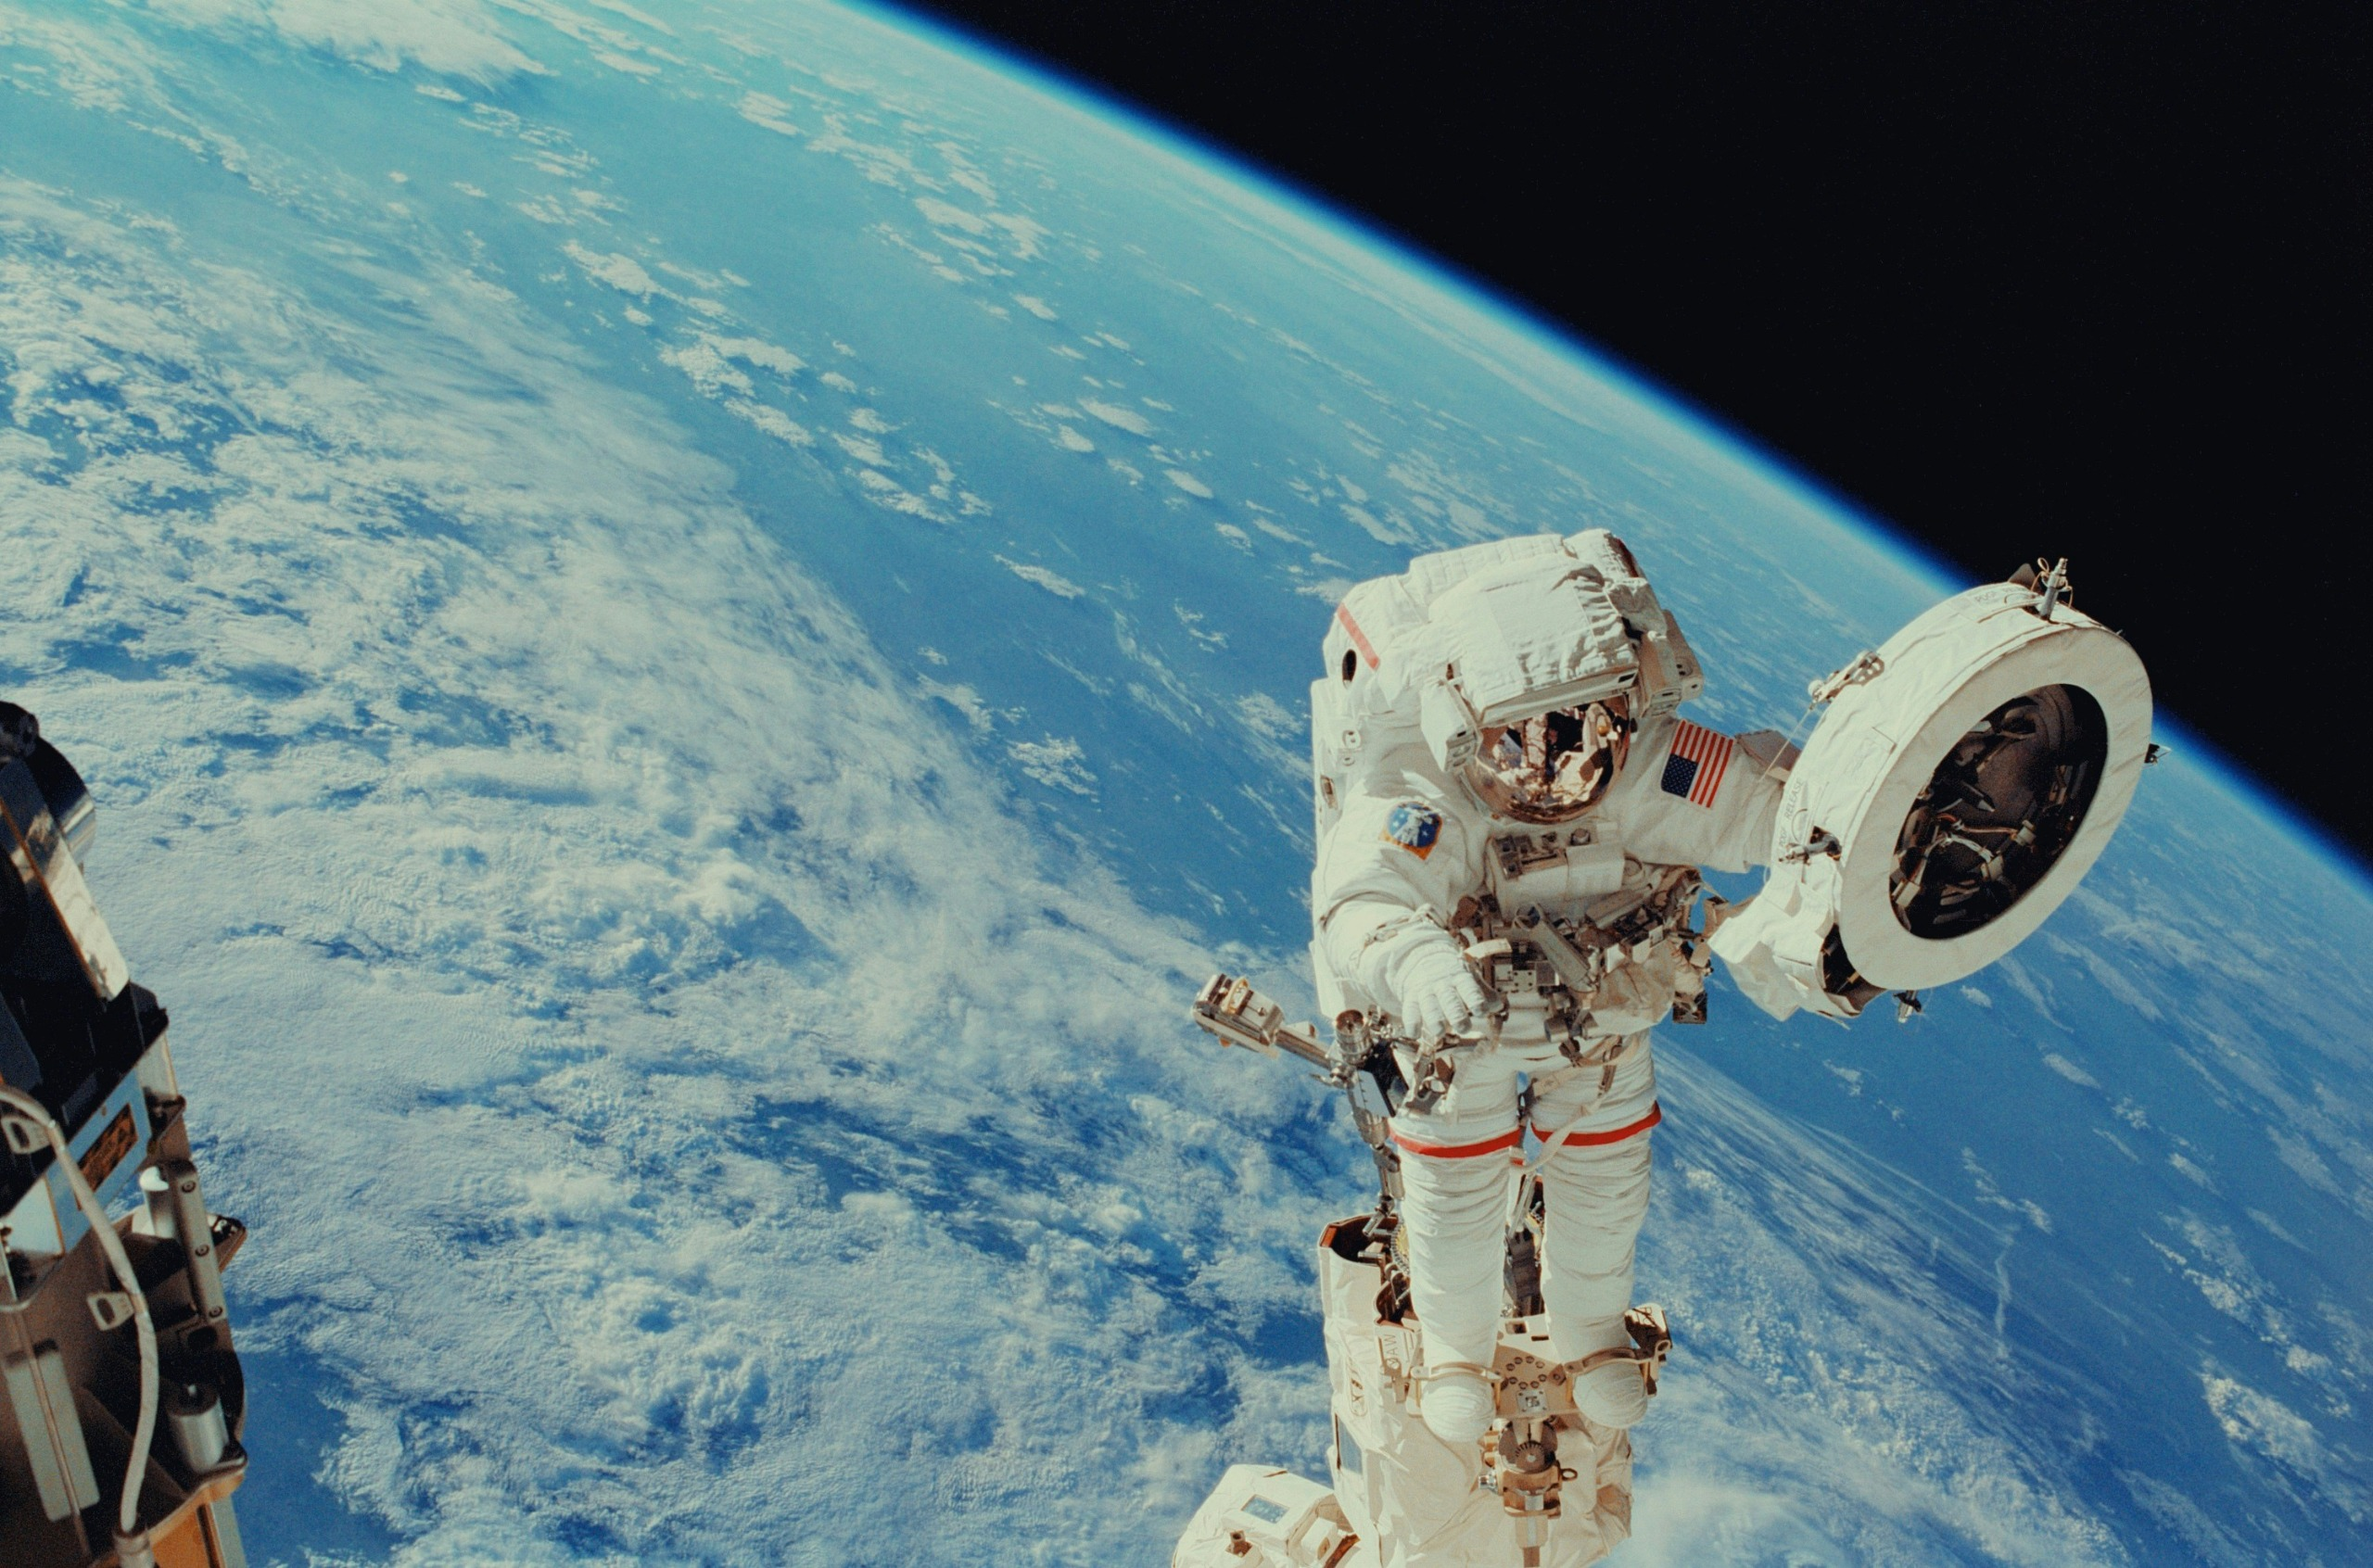
\includegraphics[height=157mm]{astrovital_portada.jpeg}};
\fill[navy,opacity=.40] (current page.north west) rectangle ([yshift=-157mm]current page.north east);
\fill[navy,opacity=.78] ([yshift=-105mm]current page.north west) rectangle ([yshift=-157mm]current page.north east);
\node[anchor=north west,text=white,font=\bfseries\large] at ([xshift=16mm,yshift=-14mm]current page.north west) {ASTROVITAL};
\node[anchor=north west,text=white,align=left,text width=178mm,font=\bfseries\fontsize{23}{27}\selectfont] at ([xshift=16mm,yshift=-112mm]current page.north west) {Salud conectada para\\misiones más seguras};
\node[anchor=north west,text=white,align=left,text width=178mm,font=\small] at ([xshift=16mm,yshift=-138mm]current page.north west) {Monitoreo, análisis y seguimiento de la salud en el espacio.};
\end{scope}
\end{tikzpicture}%
}
\vspace*{149mm}
{\color{blue}\rule{\linewidth}{1.2pt}}\vspace{1.5mm}
{\large\bfseries\color{navy}01  El reto que resolvemos}\hfill{\footnotesize\bfseries\color{blue}PROPÓSITO}\par
En misiones de larga duración, la radiación espacial, los cambios gravitacionales, el aislamiento y la distancia de la Tierra exigen mayor autonomía para observar el estado de salud. El desafío \textit{Create Health Monitoring Software for Astronauts on Space Missions} propone herramientas visuales para reconocer cambios y actuar con información comprensible.
\begin{infobox}
\textbf{Nuestra respuesta:} unificar signos vitales, historial y alertas interpretables en una plataforma que ofrece contexto científico y orientación para la tripulación, como \textbf{apoyo al seguimiento y a las decisiones}, no como diagnóstico clínico automático.
\end{infobox}
\vspace{1mm}
{\color{blue}\rule{\linewidth}{.8pt}}\vspace{1.5mm}
{\large\bfseries\color{navy}02  Propuesta de valor}\hfill{\footnotesize\bfseries\color{blue}POR QUÉ ASTROVITAL}\par\vspace{2mm}
\begin{tabularx}{\linewidth}{@{}X@{\hspace{8mm}}X@{}}
\textbf{\color{blue}Medir}\quad ECG, frecuencia cardiaca, SpO\textsubscript{2} y respiración desde los sensores. &
\textbf{\color{blue}Comprender}\quad Vigencia de lecturas, gráficos y tendencias de salud.\\[5pt]
\textbf{\color{blue}Actuar}\quad Avisos interpretables y orientación para comprobar valores. &
\textbf{\color{blue}Contextualizar}\quad Escenarios de estación, órbita, Luna y Marte con referencias NASA.\\
\end{tabularx}\par
\vfill
{\scriptsize\color{muted}Reto oficial: }\linktxt{Consultar el reto oficial}{https://www.spaceappschallenge.org/2026/challenges/health-monitoring-software/}\par
{\scriptsize\color{muted}Imagen de portada suministrada por el equipo.}
\newpage
\heading{03  Experiencia de uso}{UN SISTEMA, VARIOS MOMENTOS}
\par\noindent\begin{tabularx}{\linewidth}{@{}>{\bfseries\color{blue}}p{16mm}>{\bfseries\color{navy}}p{41mm}X@{}}
01 & Iniciar sesión & Acceso individual al panel y consulta del estado reciente de salud y del dispositivo.\\[7pt]
02 & Conectar sensores & Vinculación ESP32 por Bluetooth Low Energy, recepción de telemetría y revisión de la validez de las lecturas.\\[7pt]
03 & Registrar información & Complemento de las lecturas con registro manual, sueño, actividad y bienestar, según disponibilidad de datos.\\[7pt]
04 & Explorar tendencias & Gráficos e historial para comparar mediciones, cambios temporales y patrones de comportamiento.\\[7pt]
05 & Evaluar resultados & Motor de reglas que incorpora calidad de señal, vigencia, tendencias y ambiente seleccionado.\\[7pt]
06 & Consultar avisos & Indicaciones comprensibles, alertas y posibles acciones de verificación antes de continuar el seguimiento.\\
\end{tabularx}\par
\heading{04  Módulos del producto}{FUNCIONALIDADES}
\par\noindent\begin{tabularx}{\linewidth}{@{}X@{\hspace{6mm}}X@{}}
\begin{infobox}\tinyhead{Panel de salud}\par\textbf{Indicadores en una mirada}\par Tarjetas de pulso, SpO\textsubscript{2} y respiración; estado actual, visualización de señales y vigencia de datos.\end{infobox}&
\begin{infobox}\tinyhead{Seguimiento histórico}\par\textbf{Cambios visibles}\par Series temporales, historial de mediciones y lectura de tendencias para una evaluación personal.\end{infobox}\\[5pt]
\begin{infobox}\tinyhead{Ambiente de captura}\par\textbf{Contexto espacial}\par Escenarios de misión y referencias físicas y radiológicas para interpretar condiciones operativas.\end{infobox}&
\begin{infobox}\tinyhead{Avisos y evaluación}\par\textbf{Información explicable}\par Reglas transparentes, mensajes de atención y sugerencias de revisión de sensores o resultados.\end{infobox}\\
\end{tabularx}\par
\heading{05  Criterios de diseño}{CLARIDAD EN MISIONES EXIGENTES}
La experiencia prioriza jerarquía visual, lectura rápida, navegación responsiva, interfaces en español e inglés y diferenciación entre datos actuales y desactualizados. Un resultado ausente no se presenta como un valor cero; la interfaz comunica explícitamente la calidad de conexión y la disponibilidad de la señal.
\begin{navybox}
{\color{white}\bfseries El aporte central de ASTROVITAL}\par{\color{white}No se limita a mostrar números: reúne \textbf{captura física + registros + tendencias + reglas de decisión + contexto espacial} para facilitar el seguimiento autónomo y la comunicación de riesgos.}
\end{navybox}
\newpage
\heading{06  Arquitectura tecnológica}{DE LOS SENSORES A LA DECISIÓN}
\begin{center}
\begin{tikzpicture}[node distance=4.5mm,>=Latex,every node/.style={font=\footnotesize},mod/.style={draw=line,fill=light,rounded corners=3pt,text=navy,align=center,text width=45mm,minimum height=15mm},arr/.style={-Latex,thick,draw=blue}]
\node[mod] (a) {\textbf{ESP32 + sensores}\\ECG, pulso, SpO\textsubscript{2}, respiración};
\node[mod,right=10mm of a] (b) {\textbf{Frontend Next.js / React}\\Panel, BLE, formularios, gráficos};
\node[mod,below=8mm of b] (c) {\textbf{Backend Next.js / API}\\Autenticación y validación};
\node[mod,left=10mm of c] (d) {\textbf{PostgreSQL / Supabase}\\Usuarios, lecturas y avisos};
\node[mod,below=8mm of c] (e) {\textbf{DSS + contexto NASA}\\Reglas, tendencias y referencias};
\draw[arr] (a)--node[above]{BLE}(b);\draw[arr] (b)--node[right]{HTTPS}(c);\draw[arr,<->] (c)--(d);\draw[arr,<->] (c)--(e);
\end{tikzpicture}
\end{center}
\par\noindent\begin{tabularx}{\linewidth}{@{}>{\raggedright\arraybackslash\bfseries\color{navy}}p{40mm}X@{}}
Interfaz web & Frontend independiente en Next.js, React y TypeScript. Pantallas de astronauta, historial, conexión del equipo, registro manual, entorno y alertas.\\[5pt]
Servicios backend & API REST, manejo de sesión, validación, persistencia y servicio DSS disponible mediante \texttt{GET /api/v1/me/dss}.\\[5pt]
Persistencia & Base PostgreSQL en Supabase para perfiles, lecturas, avisos y otras entidades de la aplicación.\\[5pt]
Capa electrónica & Firmware para ESP32 con sensores y transporte BLE; herramientas de puente local y pruebas de compatibilidad.\\[5pt]
Motor de evaluación & Árbol de decisiones con reglas demostrativas que examinan indicadores, vigencia, calidad de información, contexto y posibles avisos.\\[5pt]
Despliegue y calidad & Frontend y backend publicados como servicios separados en Vercel; verificaciones de tipos, lint, compilación y pruebas de sensores y evaluación.\\
\end{tabularx}\par
\heading{07  Flujo técnico}{TRAZABILIDAD}
\begin{infobox}
\textbf{Captura} \(\rightarrow\) \textbf{recepción BLE o registro manual} \(\rightarrow\) \textbf{validación} \(\rightarrow\) \textbf{almacenamiento} \(\rightarrow\) \textbf{análisis DSS} \(\rightarrow\) \textbf{visualización y aviso}.\par
El DSS contempla lecturas ausentes o desactualizadas y evita presentar una evaluación como concluyente si no existe información suficiente. La referencia radiológica histórica caracteriza el escenario, mientras que los signos vitales del usuario provienen del ESP32 o de sus registros.
\end{infobox}
\heading{08  Evolución y potencial}{VALOR PARA EL RETO}
La solución facilita la integración progresiva de nuevas variables fisiológicas, nuevos sensores y perfiles ambientales. Su arquitectura modular separa la captura, el procesamiento y la presentación, permitiendo mejorar las reglas y añadir mecanismos de verificación sin rehacer toda la experiencia del astronauta.
\newpage
\heading{09  Datos científicos NASA}{RADIOLOGÍA ESPACIAL INCORPORADA}
El módulo ambiental trabaja con resúmenes de series históricas procedentes del \textbf{NASA Open Science Data Repository, RadLab}. Los datos permiten comparar referencias instrumentales de diferentes misiones y explicar cómo cambia la exposición radiológica según el escenario.
\par\noindent\begin{tabularx}{\linewidth}{@{}>{\bfseries\color{navy}}p{33mm}p{58mm}>{\raggedleft\arraybackslash}p{23mm}X@{}}
\toprule Escenario & Misión / instrumento & Registros & Fuente\\\midrule
Marte, superficie & Curiosity · MSL-RAD & 274.998 & \linktxt{RadLab}{https://visualization.osdr.nasa.gov/radlab/gui/overview/}\\[4pt]
Órbita lunar & LRO · CRaTER-D1D2 & 71.626 & \linktxt{RadLab}{https://visualization.osdr.nasa.gov/radlab/gui/overview/}\\[4pt]
Tránsito espacial & Artemis I · Orion EAD-MU01 & 7.303 & \linktxt{RadLab}{https://visualization.osdr.nasa.gov/radlab/gui/overview/}\\\midrule
\multicolumn{2}{@{}l}{\textbf{Total de observaciones históricas reportadas}} & \textbf{353.927} & \linktxt{API RadLab}{https://visualization.osdr.nasa.gov/radlab/gui/data-api/}\\\bottomrule
\end{tabularx}\par
\par{\footnotesize\color{muted}Unidad indicada en el resumen aportado: \(\mu\mathrm{Gy/h}\). Resúmenes documentados en \texttt{data/radlab\_reference\_summaries.json} del repositorio. Son referencias instrumentales, no dosis corporal de los usuarios. Los conteos y percentiles fueron aportados; no se reprodujeron sin los CSV originales.}
\heading{10  Fuentes NASA para el contexto ambiental}{CATÁLOGO Y REFERENCIAS}
\par\noindent\begin{tabularx}{\linewidth}{@{}>{\bfseries\color{navy}}p{43mm}X@{}}
NASA Earthdata & \linktxt{Earthdata Search}{https://search.earthdata.nasa.gov/}: portal de descubrimiento y consulta de datos de observación terrestre.\\[4pt]
Landsat & \linktxt{NASA Landsat}{https://landsat.gsfc.nasa.gov/}: programa de observación terrestre y documentación de misión.\\[4pt]
Perseverance / MEDA & \linktxt{Archivo atmosférico NASA PDS}{https://pdsatmospheres.nmsu.edu/data_and_services/atmospheres_data/PERSEVERANCE/meda.html}: condiciones meteorológicas de Marte.\\[4pt]
LRO / Diviner & \linktxt{NASA PDS Diviner}{https://pds-geosciences.wustl.edu/missions/lro/diviner.htm}: referencias térmicas de la Luna.\\[4pt]
NASA Human Research Program & \linktxt{Five Hazards of Human Spaceflight}{https://www.nasa.gov/hrp/hazards/}: factores de riesgo de la exploración humana.\\[4pt]
NASA-STD-3001 & \linktxt{Human-System Standard, Vol. 2}{https://www.nasa.gov/reference/nasa-std-3001v2/}: requisitos humanos y de salud espacial.\\[4pt]
NASA HRP, evidencia & \linktxt{Informe sobre sueño}{https://humanresearchroadmap.nasa.gov/Evidence/reports/Sleep.pdf} y \linktxt{repositorio de riesgos}{https://humanresearchroadmap.nasa.gov/}: respaldo conceptual de indicadores y riesgos.\\
\end{tabularx}\par
\begin{infobox}
\textbf{Cómo se aprovechan estas fuentes.} RadLab constituye la referencia cuantitativa radiológica del DSS. MEDA, Diviner y el Human Research Program sirven como referencias ambientales y científicas; Earthdata y Landsat se consignan como portales NASA relacionados con observación y exploración de datos, sin atribuirles una integración operativa no demostrada.
\end{infobox}
\heading{11  Interpretación y confiabilidad}{ANÁLISIS EXPLICABLE}
El árbol de decisiones combina disponibilidad de señales, rangos de referencia, evolución de lecturas y contexto de misión para comunicar observaciones y avisos. La aplicación distingue entre datos actuales, históricos y no válidos, y presenta la interpretación en lenguaje comprensible. El enfoque es de \textbf{monitoreo y orientación}, no de diagnóstico o validación médica para vuelo.
\newpage
\heading{12  Declaración de inteligencia artificial}{TRANSPARENCIA DEL PROCESO}
La inteligencia artificial generativa, \textbf{ChatGPT y Codex de OpenAI}, se empleó como herramienta de asistencia a lo largo del ciclo de desarrollo de ASTROVITAL, incluida la \textbf{generación de código}. Su participación abarcó actividades técnicas, de investigación y comunicación, con integración y decisiones finales a cargo del equipo. La creación del logotipo SVG de AstroVital también contó con asistencia de IA.
\par\noindent\begin{tabularx}{\linewidth}{@{}>{\bfseries\color{navy}}p{48mm}X@{}}
Programación y generación de código & Borradores y revisiones de componentes React, lógica TypeScript/JavaScript, servicios backend, interfaces, estructuras de datos y funciones de integración.\\[7pt]
Arquitectura de software & Apoyo en la definición de capas, comunicación ESP32-BLE-frontend, rutas API, almacenamiento y separación de responsabilidades.\\[7pt]
Modelo DSS y análisis & Diseño y mejora de reglas de decisión, interpretación de señales, manejo de estados y redacción de explicaciones de riesgos.\\[7pt]
Depuración y verificación & Análisis de fallos, propuestas de corrección, casos de prueba, razonamiento sobre telemetría y revisión de consistencia.\\[7pt]
Interfaz y experiencia & Propuestas de distribución visual, jerarquía de indicadores, mensajes de alerta, microtextos e interacciones.\\[7pt]
Documentación científica & Organización de fuentes NASA, síntesis de documentación, justificación técnica y redacción de materiales del proyecto.\\
\end{tabularx}\par
\begin{navybox}
{\color{white}\textbf{Responsabilidad del equipo.} La IA se utilizó como apoyo al diseño, programación, pruebas y documentación. ASTROVITAL fue integrado y adaptado como prototipo por sus desarrolladores, quienes asumen las decisiones de ingeniería, la revisión del código y la presentación de resultados.}
\end{navybox}
\heading{13  Visión del proyecto}{TECNOLOGÍA AL SERVICIO DE LA TRIPULACIÓN}
ASTROVITAL propone una forma accesible de observar la salud del astronauta, combinar datos personales con la complejidad de los ambientes espaciales y transformar esa información en avisos fáciles de comprender. La experiencia busca fortalecer el autocuidado y la preparación de la tripulación en misiones cada vez más prolongadas.
\vfill
{\color{blue}\rule{\linewidth}{1pt}}\vspace{3pt}
{\small\bfseries\color{navy}ASTROVITAL}\hfill{\footnotesize\color{muted}Ficha técnica del proyecto · 2026}

\newpage
\heading{14  Acceso directo a recursos y datasets}{ENLACES COMPLETOS Y CLICABLES}
Los siguientes enlaces permiten acceder directamente a la plataforma ASTROVITAL, al repositorio público y a las fuentes científicas consultadas. Se muestran las direcciones completas para facilitar su verificación y apertura en el navegador.
\begin{infobox}
\tinyhead{Producto y código fuente}\par\textbf{Plataforma desplegada}\par\url{https://astrovital-health.vercel.app/login}\par\vspace{3pt}
\textbf{Repositorio de ASTROVITAL}\par\url{https://github.com/AMVMesias/ASTROVITAL}\par\vspace{3pt}
\textbf{Licencia MIT en la raíz del repositorio}\par\url{https://github.com/AMVMesias/ASTROVITAL/blob/main/LICENSE}\par\vspace{3pt}
\textbf{Reto oficial del proyecto}\par\url{https://www.spaceappschallenge.org/2026/challenges/health-monitoring-software/}
\end{infobox}
\heading{15  NASA OSDR RadLab}{SERIES HISTÓRICAS DE RADIACIÓN}
\textbf{Fuente principal de las tres series incorporadas al DSS:} NASA Open Science Data Repository, RadLab. Los instrumentos MSL-RAD (Curiosity), CRaTER (LRO) y EAD-MU01 (Orion / Artemis I) se documentan mediante el mismo portal; no se atribuyen enlaces de descarga filtrada que no estén registrados.
\par\noindent\begin{tabularx}{\linewidth}{@{}>{\raggedright\arraybackslash\bfseries\color{navy}}p{39mm}X@{}}
Portal oficial de RadLab & \url{https://visualization.osdr.nasa.gov/radlab/gui/overview/}\\[6pt]
Gráficas y series temporales & \url{https://visualization.osdr.nasa.gov/radlab/gui/time-series-plots/}\\[6pt]
Documentación de la API & \url{https://visualization.osdr.nasa.gov/radlab/gui/data-api/}\\
\end{tabularx}
\heading{16  Otras fuentes NASA}{ARCHIVOS Y PORTALES CIENTÍFICOS}
\par\noindent\begin{tabularx}{\linewidth}{@{}>{\raggedright\arraybackslash\bfseries\color{navy}}p{40mm}X@{}}
MEDA / Perseverance & \url{https://pdsatmospheres.nmsu.edu/data_and_services/atmospheres_data/PERSEVERANCE/meda.html}\\[6pt]
DOI MEDA & \url{https://doi.org/10.17189/1522849}\\[6pt]
NASA Earthdata Search & \url{https://search.earthdata.nasa.gov/}\\[6pt]
NASA Landsat & \url{https://landsat.gsfc.nasa.gov/}\\[6pt]
LRO / Diviner & \url{https://pds-geosciences.wustl.edu/missions/lro/diviner.htm}\\
\end{tabularx}
\vfill
{\footnotesize\color{muted}Los enlaces de RadLab conducen al servicio oficial y a su explorador de series temporales. La selección exacta de filtros de los archivos históricos no está incluida en este documento.}
\newpage
\heading{17  Informes NASA sobre salud espacial}{REFERENCIAS COMPLETAS}
Estas fuentes oficiales fundamentan la explicación de riesgos cardiovasculares, descompresión, lesiones durante actividad extravehicular, capacidad física y sueño. Las URL son clicables y se reproducen completas.
\renewcommand{\arraystretch}{1.13}
\begin{infobox}
\tinyhead{Estándar de salud de referencia}\par
\textbf{NASA-STD-3001, Volumen 2}\par
\url{https://www.nasa.gov/reference/nasa-std-3001v2/}
\end{infobox}
\vspace{3pt}
{\small\bfseries\color{navy}Riesgos cardiovasculares}\par
{\footnotesize\url{https://humanresearchroadmap.nasa.gov/Evidence/reports/Cardio%20Risk%20EB%202022%20FINAL_4-3-2023.pdf}}\par\vspace{6pt}
{\small\bfseries\color{navy}Lesiones durante actividad extravehicular (EVA)}\par
{\footnotesize\url{https://humanresearchroadmap.nasa.gov/Evidence/other/EVA%20Injury%20Evidence%20Report%20FINAL_6-14-2023.pdf}}\par\vspace{6pt}
{\small\bfseries\color{navy}Hipoxia y enfermedad por descompresión}\par
{\footnotesize\url{https://humanresearchroadmap.nasa.gov/Evidence/other/Evidence%20Report%20Hypoxia%20and%20DCS_FINAL_1-8-2024.pdf}}\par\vspace{6pt}
{\small\bfseries\color{navy}Capacidad aeróbica y muscular}\par
{\footnotesize\url{https://humanresearchroadmap.nasa.gov/Evidence/reports/Evidence%20report%20aerobic%20and%20muscle_FINAL%204-3-2024.pdf}}\par\vspace{6pt}
{\small\bfseries\color{navy}Pérdida de sueño y alteraciones del descanso}\par
{\footnotesize\url{https://humanresearchroadmap.nasa.gov/Evidence/reports/Sleep.pdf}}\par\vspace{6pt}
{\small\bfseries\color{navy}Riesgos médicos generales — NASA Human Research Roadmap}\par
{\footnotesize\url{https://humanresearchroadmap.nasa.gov/Risks/print/?i=95}}\par
\vfill
\begin{navybox}
{\color{white}\bfseries ASTROVITAL: salud conectada para misiones más seguras}\par
{\color{white}Un sistema de seguimiento que reúne señales biométricas, indicadores históricos y conocimiento espacial en una experiencia comprensible para la tripulación.}
\end{navybox}

\newpage
\heading{18  Créditos de imágenes}{FOTOGRAFÍAS Y FUENTES}
El proyecto utiliza fotografías publicadas por NASA en Unsplash. A continuación se enlazan el perfil y las páginas individuales de cada imagen.
\begin{infobox}
\textbf{Perfil de NASA en Unsplash}\par
\url{https://unsplash.com/es/@nasa}\par
\end{infobox}
\vspace{5pt}
{\small\bfseries\color{navy}Vista de la Tierra y satélite}\par
\href{https://unsplash.com/es/fotos/vista-de-la-tierra-y-satelite-yZygONrUBe8}{\textcolor{blue}{\nolinkurl{https://unsplash.com/photos/yZygONrUBe8}}}\par
\vspace{5pt}
{\small\bfseries\color{navy}Lanzamiento del cohete Soyuz}\par
\href{https://unsplash.com/es/fotos/el-cohete-soyuz-se-lanza-desde-la-plataforma-de-lanzamiento-de-baikonur-JkaKy_77wF8}{\textcolor{blue}{\nolinkurl{https://unsplash.com/photos/JkaKy_77wF8}}}\par
\vspace{5pt}
{\small\bfseries\color{navy}Astronauta junto al satélite}\par
\href{https://unsplash.com/es/fotos/fotografia-de-un-astronauta-junto-al-satelite-OLlj17tUZnU}{\textcolor{blue}{\nolinkurl{https://unsplash.com/photos/OLlj17tUZnU}}}\par
\vspace{5pt}
{\small\bfseries\color{navy}Astronauta en la Luna junto a la bandera}\par
\href{https://unsplash.com/es/fotos/astronauta-de-pie-en-la-luna-junto-a-la-bandera-de-eeuu-U2uKrI4lci8}{\textcolor{blue}{\nolinkurl{https://unsplash.com/photos/U2uKrI4lci8}}}\par
\vspace{5pt}
{\small\bfseries\color{navy}Actividad extravehicular}\par
\href{https://unsplash.com/es/fotos/astronauta-de-la-nasa-realiza-actividad-extravehicular-gYwfpVI2JzM}{\textcolor{blue}{\nolinkurl{https://unsplash.com/photos/gYwfpVI2JzM}}}\par
\vspace{8pt}
\textbf{Licencia de Unsplash:} \url{https://unsplash.com/license}

\newpage
\heading{19  Adquisición y contrato de datos}{IMPLEMENTACIÓN VERIFICABLE}
\textbf{Hardware contemplado por el software.} AD8232 para señal ECG y frecuencia estimada; MAX30102 para SpO\textsubscript{2} y pulso óptico; MPU6050 para estimación respiratoria por movimiento. Estos nombres describen el contrato implementado, no acreditan cableado, calibración ni firmware efectivamente instalado.
\begin{infobox}
\textbf{Ruta web:} ESP32 $\rightarrow$ notificaciones BLE $\rightarrow$ navegador $\rightarrow$ API Next.js $\rightarrow$ PostgreSQL/Supabase.\par
\textbf{Alternativa local:} ESP32 $\rightarrow$ Python/Bleak $\rightarrow$ API. Su cola SQLite conserva reintentos locales y no reemplaza la base del backend.
\end{infobox}
\textbf{Contrato CSV-11.} Cada línea contiene once campos numéricos, en este orden:
\begin{quote}\small\ttfamily ecg, bpm\_ecg, estado\_ecg\_x50, resp\_mg, rpm,\\ estado\_resp\_x50, spo2, bpm\_oxi, estado\_oxi\_x50, ir, rojo\end{quote}
El navegador reconstruye fragmentos hasta un salto de línea. Rechaza columnas vacías, números no finitos, estados no admitidos, UTF-8 inválido y acumulaciones superiores a 16 KiB. El modo de dos copias comprueba igualdad de fragmentos; se activa solo si el firmware realmente los duplica.
\heading{19.1  Calidad, tiempo y envío}{LÍMITES DEL TRANSPORTE}
Se envía como máximo una instantánea por segundo. Se deriva una medición de pulso cuando el estado ECG es 100 y el valor cumple el formato de 1 a 300 lpm. Sin contacto o sin señal se conserva telemetría y estado sin inventar un pulso de cero. Los rangos de formato no son intervalos fisiológicos de normalidad.

La fecha de captura web procede del reloj receptor, no de un reloj ADC sincronizado. La cola web conserva hasta diez paquetes pendientes en memoria, con un envío simultáneo y hasta tres intentos por paquete. Se mantienen los identificadores al reintentar; el backend detecta duplicados y conflictos de contenido. Cerrar o recargar puede perder pendientes no confirmados.

El monitor ECG web conserva hasta diez segundos y 3000 muestras antes del muestreo de la API. La escala utiliza unidades crudas, no milivoltios calibrados. El filtro es visual: no determina latidos ni altera registros guardados. Las instantáneas del backend no reconstruyen la onda de alta frecuencia.
\vfill
{\footnotesize\color{muted}Evidencia: \path{features/capture/protocol.ts}, \path{BleCapture.tsx}, \path{ecgStream.ts}; \path{docs/CAPTURA_BLE_WEB.md}, \path{docs/PUENTE_ESP32.md}. Rutas de frontend relativas a \path{src/frontend/src/frontend/}.}
\newpage
\heading{20  Método de evaluación}{DOS ANÁLISIS COMPLEMENTARIOS}
\textbf{Referencia personal.} Se comparan mediciones de la misma persona, misión, indicador, unidad, actividad y revisión ambiental. Se separan registros simulados de no simulados y se eliminan IDs repetidos. Para pulso se exige reposo confirmado. Fecha futura, mala calidad o caducidad impiden una evaluación vigente.
\par\noindent\begin{tabularx}{\linewidth}{@{}lXXX@{}}
\toprule Parámetro & Pulso en reposo & Sueño & Bienestar\\\midrule
Ventana histórica & 14 días & 14 días & 14 días\\
Referencia mínima & 5 muestras & 5 muestras & 5 muestras\\
Lecturas consecutivas & 3 & 3 & 3\\
Desviación absoluta & 15 lpm & 1,5 h & 1 punto\\
Vigencia máxima & 30 s & 2 días & 2 días\\\bottomrule
\end{tabularx}\par
La media de referencia excluye el bloque de tres lecturas evaluado. Para cada una, $\Delta_i=x_i-\bar{x}_{ref}$. Hay desviación sostenida si las tres diferencias alcanzan el umbral positivo o las tres son como máximo su negativo. Sin referencia suficiente se informa insuficiencia; no se afirma estabilidad. Versiones: \texttt{demo-heart-rate-rest-2}, \texttt{demo-sleep-1}, \texttt{demo-wellbeing-1}.
\heading{20.1  DSS de telemetría}{CALIDAD ANTES DE INTERPRETACIÓN}
El servicio consulta hasta 100 instantáneas desde el comienzo de la asignación ambiental activa hasta el reloj de consulta. El árbol separa dispositivos, descarta fechas futuras e IDs repetidos y exige estados válidos del firmware. La ventana de tendencias es de hasta 120 segundos; la última muestra caduca a los 30 segundos. Conservar historia no renueva la vigencia.
\begin{itemize}
\item SpO\textsubscript{2} menor de 90: prioridad de verificación. De 90 a menos de 95: revisión. Cero sin estado válido: dato no disponible.
\item ECG: con cinco valores válidos recientes como mínimo, compara la mediana de los dos más nuevos con la de los restantes. Una diferencia absoluta de al menos 20 lpm activa revisión.
\item Diferencia ECG/oxímetro de al menos 20 lpm: comprobar coherencia. Pulso óptico en el techo de formato de 300 lpm o salto de al menos 40 lpm en hasta 10 segundos: comprobar señal.
\item Respiración: informa valor y variación, sin clasificación clínica de normalidad. La radiación histórica no modifica el nivel fisiológico.
\end{itemize}
\begin{infobox}\textbf{Procedencia:} constantes demostrativas del código, no umbrales validados por NASA ni por ensayos clínicos del montaje. FDA y MedlinePlus se enlazan como orientación de comprobación, no como validación de estos parámetros.\end{infobox}
{\footnotesize\color{muted}Evidencia: \path{AssessmentService.ts}, \path{assessMeasurements.ts}, \path{telemetryDecisionTree.ts}, \path{TelemetryDecisionService.ts}, en \path{application/assessment} del backend.}
\newpage
\heading{21  Caso reproducible y trazabilidad}{DATOS SINTÉTICOS DE PRUEBA}
Ejemplo de \path{tests/telemetry-decision-tree.test.ts}, no un registro humano ni evidencia de precisión del sensor. Dos instantáneas sintéticas del mismo dispositivo y escenario, a 15 y 30 segundos antes del reloj evaluador:
\par\noindent\begin{tabularx}{\linewidth}{@{}lXX@{}}
\toprule Campo & Más reciente & Anterior\\\midrule
SpO\textsubscript{2} & 80 \% & 78 \%\\
Pulso óptico & 300 lpm & 17 lpm\\
Estado del oxímetro & 200 & 200\\
Pulso ECG / estado & 0 / 50 & 76 / 100\\
Respiración / estado & 0 / 50 & 17 / 100\\\bottomrule
\end{tabularx}\par
\begin{enumerate}[leftmargin=5mm,itemsep=5pt]
\item \textbf{Validación:} la última lectura es vigente. El estado óptico permite analizar SpO\textsubscript{2} y pulso. ECG y respiración actuales quedan no disponibles; sus ceros no son mediciones humanas.
\item \textbf{Evaluación:} resultado \texttt{priority} por SpO\textsubscript{2} de 80 \%. Pulso de 300 lpm: \texttt{review} y \texttt{checkRequired} por coincidir con el techo de formato.
\item \textbf{Acciones:} verificar oxigenación, contrastar pulso y recuperar ECG y respiración. La duda de calidad del pulso no elimina la prioridad de la saturación.
\item \textbf{Caducidad:} otra prueba con la última muestra a 31 segundos devuelve \texttt{insufficient}; retira advertencias fisiológicas actuales y solicita recuperar captura.
\end{enumerate}
El DSS de telemetría calcula resultados al consultar. Los avisos persistidos de mediciones personales siguen otra ruta: conservan ID de medición, regla, referencia, dirección y evidencia histórica. Admiten estados abierto, en seguimiento y cerrado. La agrupación visual no borra detecciones originales.
\heading{21.1  Seguridad y privacidad}{CONTROLES IMPLEMENTADOS}
La API exige sesión y permisos por rol. El propietario se resuelve desde la cuenta o vínculo del dispositivo; las consultas filtran por identidad y la captura valida el origen autorizado. Contraseñas y respuestas de recuperación usan hashes scrypt con sal. La cookie es HttpOnly, SameSite estricto y Secure en Vercel.

PostgreSQL/Supabase conserva cuentas, sesiones, mediciones, telemetría y seguimiento. El idioma y tema se guardan localmente. Cerrar sesión no elimina el historial; no se declara borrado automático ni certificación de privacidad. Estos controles no sustituyen una auditoría de seguridad o evaluación normativa.
\vfill
{\footnotesize\color{muted}Evidencia: \path{application/alerts}, \path{infrastructure/security/credentials.ts}, \path{transport/http.ts}; ingesta y permisos en \path{tests/cloud.test.ts}.}
\newpage
\heading{22  Verificación y resultados}{EJECUCIÓN DEL 15 NOVIEMBRE 2026}
Se ejecutó \texttt{npm test} sobre la base \texttt{b2daf00}, antes de ampliar este documento: \textbf{59 pruebas registradas, 58 aprobadas, 0 fallidas y 1 omitida}. La integración PostgreSQL se omitió por no disponer de \texttt{DATABASE\_URL} en esa ejecución; no acredita conexión real con Supabase.
\par\noindent\begin{tabularx}{\linewidth}{@{}>{\bfseries}p{35mm}X@{}}
\toprule Área & Cobertura observada\\\midrule
Captura BLE & Fragmentos, duplicados, once campos, UTF-8, desbordamiento, ausencia de contacto y estados.\\[6pt]
Evaluación personal & Calidad, caducidad, referencia separada, reposo confirmado y aislamiento de personas, entorno y simulación.\\[6pt]
DSS & Fechas futuras, intervalos ambientales, duplicados, dispositivos, prioridades, acciones y ausencia de influencia radiológica en el estado fisiológico.\\[6pt]
Presentación & Pulso histórico frente a actual, señal intermitente, segmentos ECG, filtro visual, grupos de avisos y eje temporal.\\[6pt]
Servicio DSS & Dependencias simuladas para permisos, asignación histórica y desconexión; no reemplazan integración real de base de datos.\\\bottomrule
\end{tabularx}\par
\textbf{Reproducción:} usar Node 22 compatible, instalar con \texttt{npm ci} y ejecutar \texttt{npm test}. La integración de \path{tests/cloud.test.ts} necesita una base de prueba autorizada y crea un esquema temporal. No publicar credenciales. Compilación y tipos son controles de software, no ensayos biomédicos.
\heading{22.1  Uso NASA y alcance de evidencia}{REFERENCIAS TRAZABLES}
El DSS importa \path{data/radlab_reference_summaries.json}. Son resúmenes suministrados: sin CSV originales no se reproduce limpieza, unidades de origen ni percentiles. CRaTER es orbital, MSL-RAD mide en Curiosity y EAD-MU01 en Orion; no son dosis del astronauta. Las fichas planetarias aportan valores documentales al catálogo. MEDA y Diviner no son flujos en vivo integrados.
\heading{22.2  Limitaciones y siguientes validaciones}{TRABAJO PENDIENTE}
\begin{itemize}
\item Documentar placa, pines, alimentación, colocación y versión real del firmware. No se añade un esquema eléctrico no verificado.
\item Comparar contra instrumentos de referencia y registrar error, condiciones y tamaño de muestra. No se acredita calibración ni validación clínica.
\item Probar captura física prolongada, movimiento, reconexión, pérdida de Internet y navegadores; registrar fallos y recuperación.
\item Recuperar CSV y metadatos originales para reproducir resúmenes; evaluar seguridad, privacidad y operación antes de uso fuera de demostración.
\end{itemize}
{\footnotesize\color{muted}Código y pruebas: \url{https://github.com/AMVMesias/ASTROVITAL}. Se distingue implementación, prueba automatizada y validación física pendiente.}

\end{document}
